\section{Environment Setup}

note: I use linux9 to run this code, please don't use linux2-4. 

The big picture about NVDLA Hardware integrator is shown in Fig.\ref{fig:hw}: 

\begin{figure}[htb]
\center
    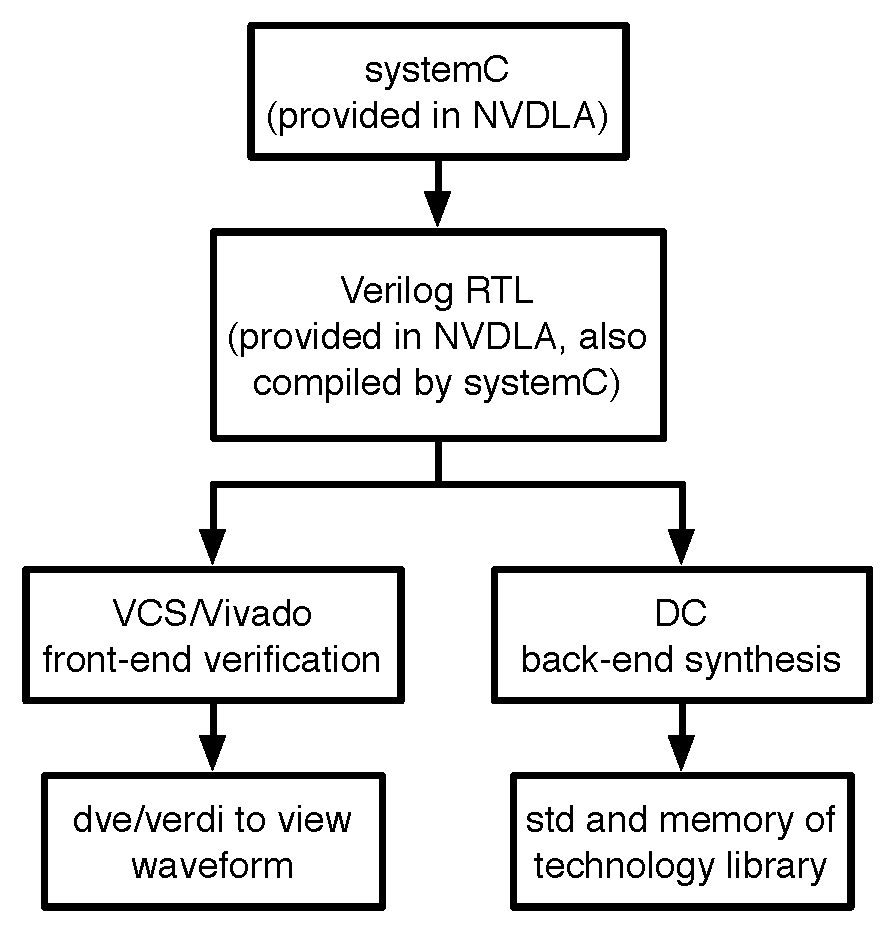
\includegraphics[width=.5\textwidth]{hw-arch}
    \label{fig:hw}
    \caption{Hardware process for NVDLA}
\end{figure}

\begin{itemize}
    \item Java - jdk1.7 (installed in "/usr/bin/java")
    %\alert{Simulation}\\ 
    \item Perl - perl-5.10 (installed in "/usr/bin/perl")\\
	XML::Simple\\
	Capture::Tiny 
    \item CPP - gcc-4.9.3 (installed in "/usr/bin/g++"")
    \item CPP (installed in "/usr/bin/cpp")
    \item Python - python2.6 (installed in "/usr/bin/python")
    \item SystemC - systemc-2.3.0 (need to be installed, by "./configure --prefix" to install in local)
    \item Verilator - Verilator 3.912 (for Verilator builds, need to be installed, by "./configure --prefix" to install in local)
    \item clang - clang 3.4 (for Verilator builds, installed in "/usr/bin/clang" in linux2-4)
\end{itemize}

Additional tools:
\begin{itemize}
    \item cpan (installed, however you have to reconfigurate installation in local dir and collect all add URL:https://metacpan.org)
    %\alert{Simulation}\\ 
    \item IO::Tee (run cpan IO::Tee to install)
    \item VCS (installed in "/opt2/synopsys/vcs-F-2011.12/bin")
    \item Verdi (installed in "/opt2/synopsys/verdi/Verdi\_M-2017.03-SP2-2/bin")
\end{itemize}

\section{Tree Build}
Revise the Makefile in hw root: 
\begin{itemize}
    \item DEFAULT\_CPP  :=  /usr/bin/cpp
    %\alert{Simulation}\\ 
    \item DEFAULT\_GCC  :=  /research/byu1/thchen/tools/gcc4.9.3/bin/g++
    \item DEFAULT\_PERL :=  /usr/bin/perl
    \item DEFAULT\_JAVA := /usr/bin/java
    \item DEFAULT\_SYSTEMC := /uac/gds/thchen/systemc/
    \item DEFAULT\_VERILATOR := /research/byu1/thchen/tools/verilator-3.9.12/bin/verilator
    \item DEFAULT\_CLANG  := /research/byu1/thchen/tools/build/bin/clang
\end{itemize}

Until now, you can run in hw root:
\begin{itemize}
    \item make
    %\alert{Simulation}\\ 
    \item ./tools/bin/tmake -build vmod
    \item ./tools/bin/tmake -build verif\_sim
    \item ./tools/bin/tmake -build cmod\_top
\end{itemize}

\section{Front-end Verification}
Next, we will compile Verilog RTL code and generate waveform.

If you want to use VCS to compile verilog RTL, you will revise the Makefile in hw-root/verif/sim/
\begin{itemize}
    \item export VCS\_HOMW := /opt2/synopsys/vcs-F-2011.12
    %\alert{Simulation}\\ 
    \item export VERDI\_HOME := /opt2/synopsys/verdi/Verdi\_M-2017.03-SP2-2
    \item export NOVAS\_HOME := /opt2/synopsys/verdi/Verdi\_M-2017.03-SP2-2
    \item export LM\_LICENSE\_FILE := /opt2/synopsys/key
    \item export VCS\_CC := /usr/bin/g++
\end{itemize}

Until now, you can run in hw-root/verif/sim
\begin{itemize}
    \item make build
    %\alert{Simulation}\\ 
    \item make run TESTDIR=../traces/traceplayer/sanity0
    \item make build DUMP=1 DUMPER=VERDI
    \item make vericom DUMP=1 DUMPER=VERDI
    \item make run DUMP=1 DUMPER=VERDI TESTDIR=../traces/traceplayer/sanity0
    \item make verdi DUMP=1 DUMPER=VERDI TESTDIR=../traces/traceplayer/sanity0
\end{itemize}


If you want to use vivado to compile verilog RTL, you will revise the Makefile in hw-root/verif/sim\_vivado
\begin{itemize}
    \item export XILINX\_HOME := /research/byu1/thchen/tools/vivado0/Vivado/2017.1
    %\alert{Simulation}\\ 
    \item PERL := /bin/perl
    \item AWK := /bin/awk
    \item TEE := /bin/tee
\end{itemize}
Until now, you can run in hw-root/verif/sim\_vivado
\begin{itemize}
    \item make build
    %\alert{Simulation}\\ 
    \item make run TESTDIR=../traces/traceplayer/sanity0
    \item make run GUI=1 TESTDIR=../traces/traceplayer/sanity0
    \item make build DUMP=1
    \item make run DUMP=1 TESTDIR=../traces/traceplayer/sanity0
    \item make regress
    \item make regress MINIREGRESS=1
\end{itemize}

\section{Back-end Synthesis}
To be up-dated soon...



\section*{Acknowledge}
I many thank Yuzhe Ma@CSE, CUHK and Zhenyu Zhu@IC school, SEU/Nanrui Micro give help for building this environment. 

\section{Reference}
1. NVDLA, http://nvdla.org